\section{Wprowadzenie}

\begin{frame}
     \frametitle{Domain Specific Languages (DSL)}
     
     DSL to języki przystosowane do używania w konkretnym celu.
     \begin{itemize}
          \item
          łatwość użycia
          \item
          specyficzne konstrukcje
          \item 
          ograniczone możliwości
          \item
          kompilacja do języka niższego poziomu (np. SQL)
     \end{itemize}


\end{frame}



\begin{frame}
\frametitle{Sumerologia}
\begin{columns}
 \column{0.5\textwidth}
Sumerologia to nauka badająca kulturę i historię starożytnych Sumerów, czerpiąca wiedzę m.in. z zachowanych tabliczek.
\begin{itemize}
\item zdigitalizowane i ręcznie skorygowane treści tabliczek są udostępnione przez system CDLI (obecnie prawie 225 000 tabliczek)
\item możliwość niewłaściwej interpretacji klinów
\item potrzebne intuicyjne narzędzie do wyszukiwania w bazie tabliczek na podstawie odczytów
\end{itemize} 
 \column{0.5\textwidth}
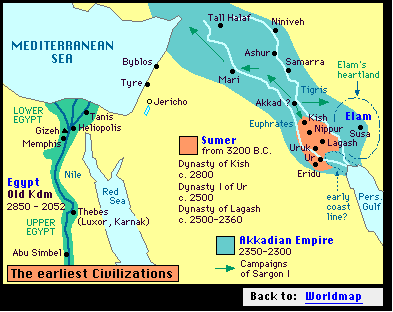
\includegraphics[width=55mm]{../1/sum_map.png}
\end{columns}
\end{frame}


\begin{frame}
     \frametitle{Tablets Query Language}
 \begin{columns}
 \column{0.5\textwidth}
   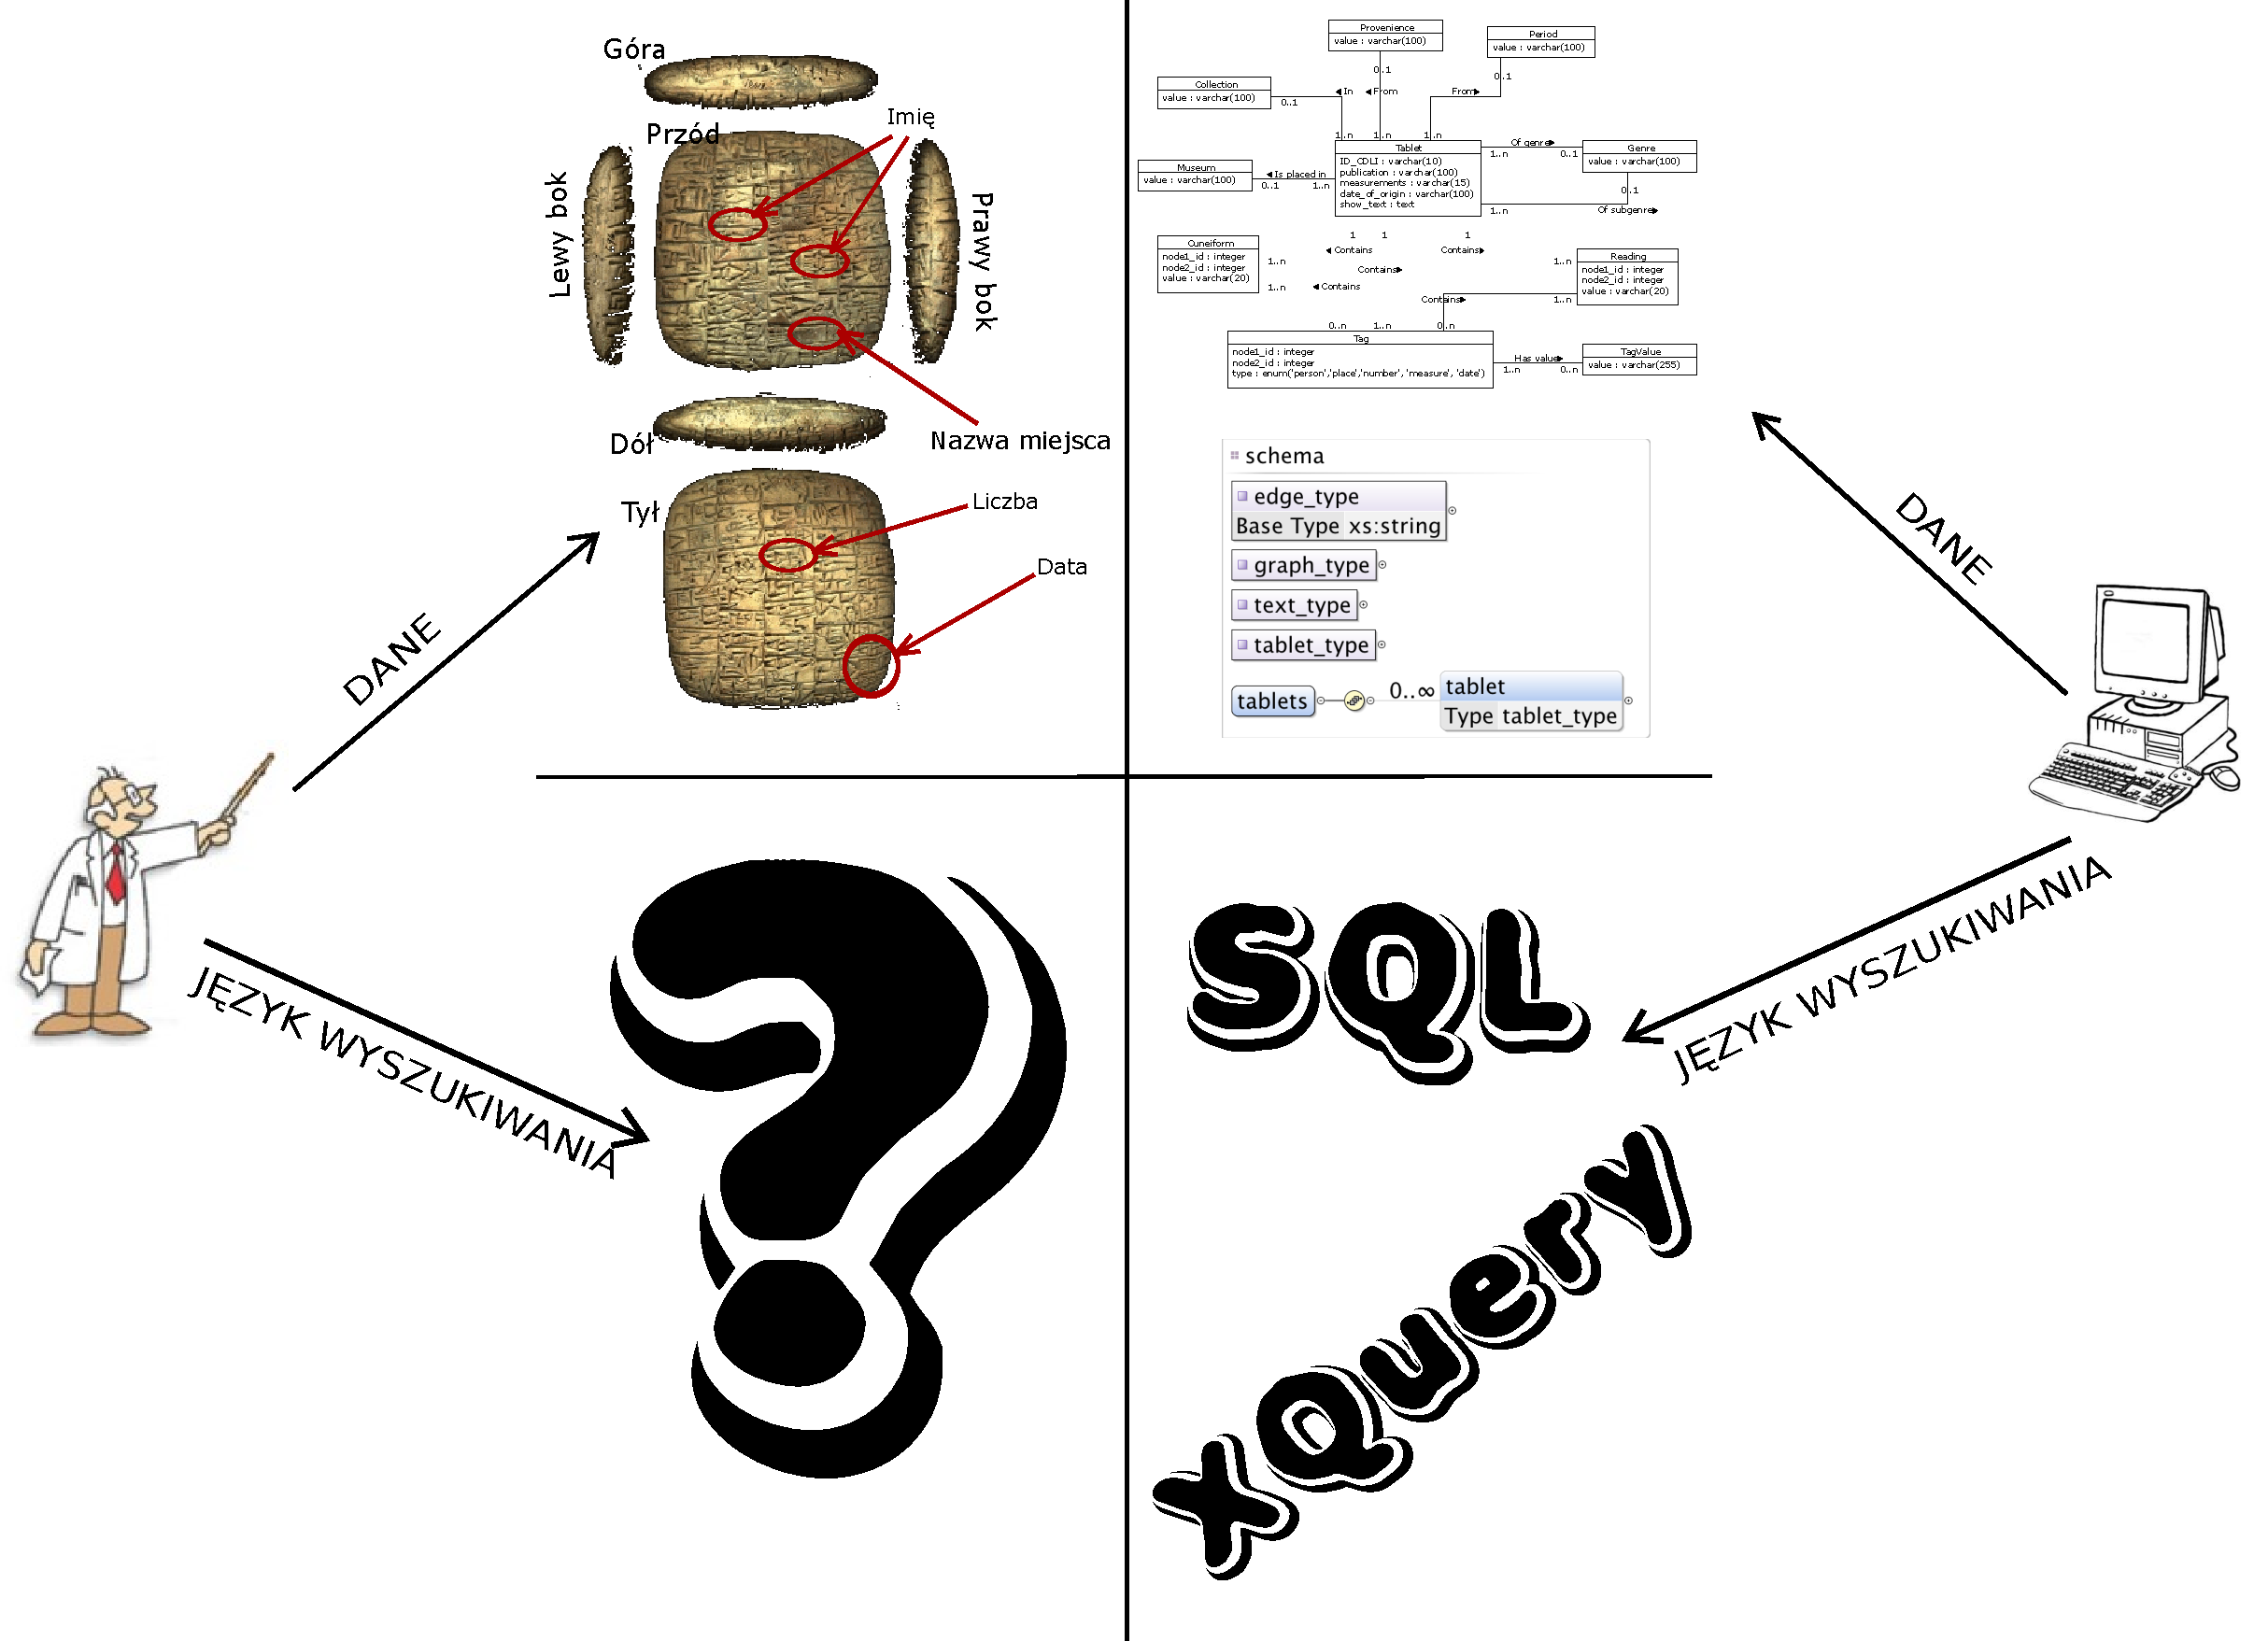
\includegraphics[width=55mm]{../diagramy/poco.pdf}      
 \column{0.5\textwidth}
  \begin{itemize}
    \item Język pozwalający sumerologom łatwo tworzyć zapytania w bazie tabliczek.\\
    \item  Prosta składnia zapytań.\\
    \item    Zapytania zawierają informacje tylko o treści tabliczek i ich metadanych.\\
    \item   Możliwość stworzenia implementacji na dowolną bazę przechowującą tabliczki.\\ %ułatwiamy to dzięki podziałowi kodu na moduły
  \end{itemize}
 \end{columns}
\end{frame}

\begin{frame}
 \frametitle{Przykładowe zapytanie TQL}
\begin{block}{Przykład}
\textbf{define}\\
~~provenience: Garshana\\
~~text: "udu ban"/mash2\\
\textbf{as} "zwierzaki w Garshana"\\
~\\
\textbf{search}\\
~~period: UrIII\\
~~text: szid + sipa $--$ adad-tilati\\
\textbf{in} "zwierzaki w Garshana"\\
~\\
\textbf{search}\\
~~period: UrIV\\
~~genre: Adm*\\
\textbf{in} "zwierzaki w Garshana"\\
\end{block}
\end{frame}
